\documentclass[12pt]{beamer}
\usepackage[english]{babel}
\usetheme[progressbar=frametitle]{metropolis}
\usetikzlibrary{positioning}
\usepackage{appendixnumberbeamer}
\usepackage{booktabs}
\usepackage{pgfplots}
\usepgfplotslibrary{dateplot}
\usepackage{xspace}
\newcommand{\themename}{\textbf{\textsc{metropolis}}\xspace}
\usepackage[font=scriptsize]{caption}
\usepackage[utf8]{inputenc}
%images
\usepackage{graphicx}
\graphicspath{ {./images/} }
%bullet points
\usepackage{listings}
\usepackage{lstautogobble}



\title{Game Design with \\ Answer Set Programming}
\subtitle{DaBlocksWorld}
\author{Dario Klepoch}
\date{17.03.2020}
\institute{Universität Potsdam}

\begin{document}
    %setting code style
    \lstset{
        language=prolog,
        autogobble=true 
    }

    \maketitle

    \begin{frame}[fragile]{AI-based Game Design}
        ``the development of innovative artificial intelligence systems plays a crucial role
        in the exploration of currently unreachable [game design] spaces.''
        \newline
        \newline
        \newline
        \newline
        \tiny{Elad hari et al. (2011)}
    \end{frame}
    
    \begin{frame}[fragile]{Contents}
        \tableofcontents[hidesubsections]
    \end{frame}


    \section{Godot}
        \begin{frame}[fragile]{Godot}
           \begin{itemize}
               \item Open source game engine
               \item Provides tool set for 2D/3D development
               \item Under MIT license
               \item Written in C/C++
               \item Used for this project
               \item Supports C/C++/C\#/GodotScript 
           \end{itemize} 
        \end{frame}

    \section{Blocks World Planning Problem}
        \begin{frame}[fragile]{BWPP}
           \begin{itemize}
               \item Blocks World Planning Problem (BWPP)
               \item Consists of Blocks
               \item Can be placed on the ground
               \item Or on another Block (creates Stack)
               \item Has start-configuration and goal-configuration
               \item Goal:
               \begin{itemize}
                   \item Convert start-config to goal-config (with few moves)
               \end{itemize}
                \item Ambiguous BWPP configurations exist
           \end{itemize} 
        \end{frame}

        \begin{frame}[fragile]
            \frametitle{Start-config}
            \begin{figure}
                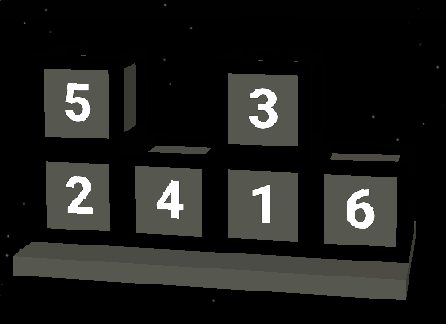
\includegraphics[width=9cm]{start_config.png}
            \end{figure} 
        \end{frame}
        
        \begin{frame}[fragile]
            \frametitle{Start-/goal-config}
            \begin{figure}
                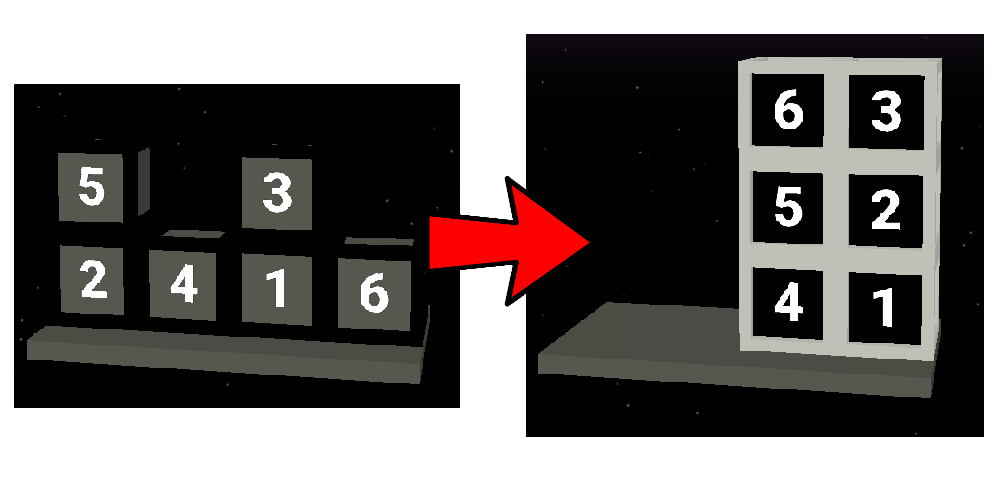
\includegraphics[width=\linewidth]{start_goal_config.png}
            \end{figure} 
        \end{frame}
        
        \begin{frame}[fragile]
            \frametitle{Ambiguous goal-config}
            \begin{figure}
                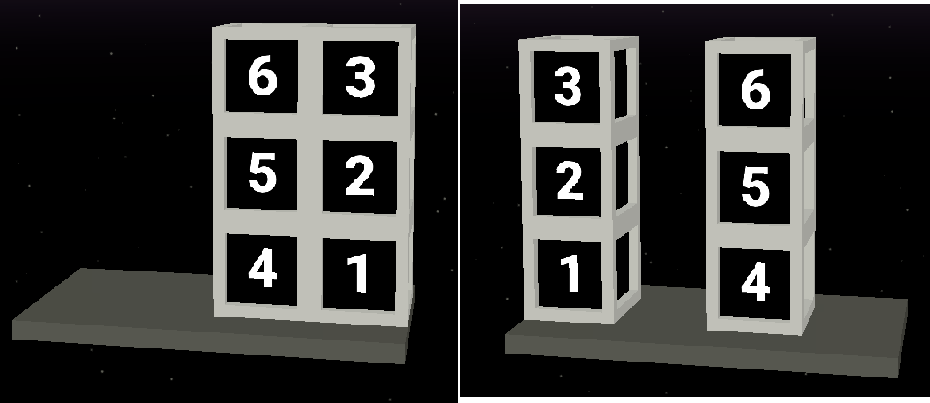
\includegraphics[width=\linewidth]{ambiguous_goal_config.png}
            \end{figure} 
        \end{frame}

        \begin{frame}[fragile]{Rules for moves}
            \begin{itemize}
                \item Legal moves follow these rules:
                \begin{itemize}
                    \item No other block on the moved block
                    \item Only one block can be moved at one time point
                    \item Block can be moved to the ground (without limit)
                \end{itemize}
            \end{itemize}
        \end{frame}

    \section{Game Design}
        \begin{frame}[fragile]{What is DaBlocksWorld?}
            \begin{itemize}
                \item Is an interactive implementation of BWPP
                \item The differences are: 
                \begin{itemize}
                    \item Blocks cannot be moved unlimited to the ground
                    \item Blocks cannot be stacked unlimited
                    \item Width and height match optimal plan
                    \item Numbers are limited
                    \item Stacks are marked by colors
                \end{itemize}
                \item Developed in Godot
                \item Uses Clingo for inference tasks
            \end{itemize}
        \end{frame}

        \begin{frame}[fragile]
            \frametitle{Changed rules}
            \begin{figure}
                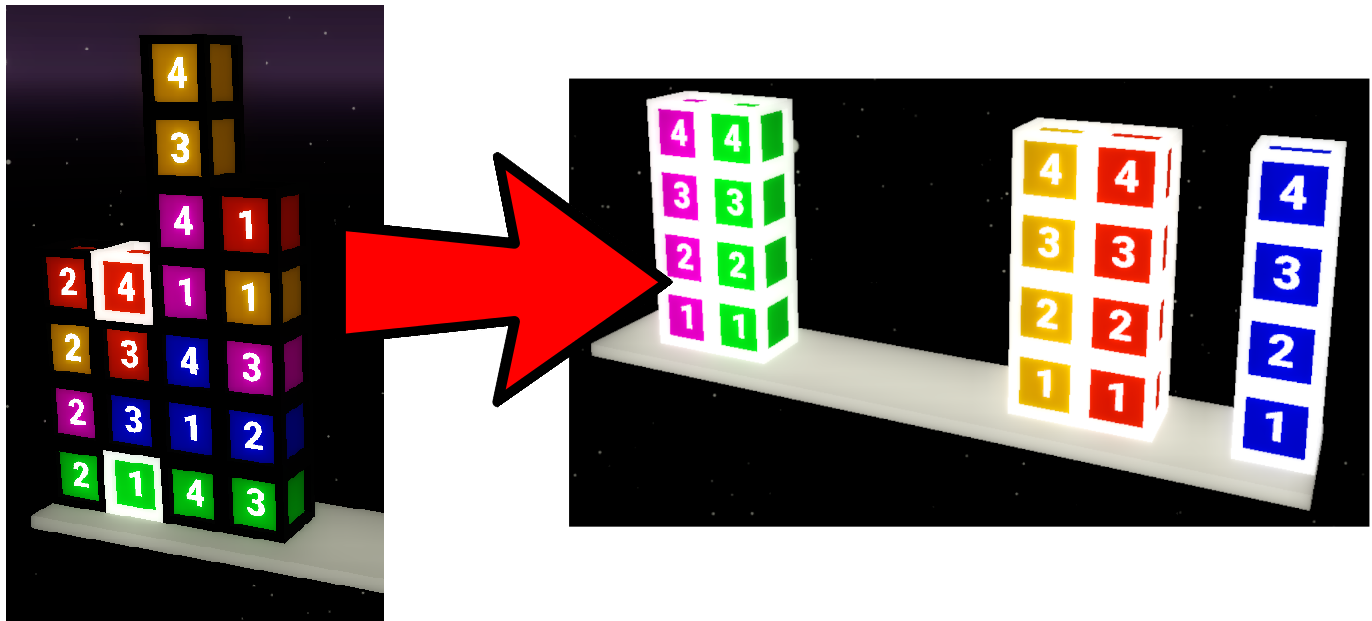
\includegraphics[width=\linewidth]{start_goal_config_colored.png}
            \end{figure} 
        \end{frame}

        \begin{frame}[fragile]{Game Loop of DaBlocksWorld}
            \begin{itemize}
                \item Player selects difficulty
                \item Random configuration will be generated
                \item Translate configuration to Clingo atoms
                \item Solve with Clingo
                \item Let player beat the level
                \item Rate player based on the number of optimal moves
            \end{itemize}
        \end{frame}

        \begin{frame}[fragile]
            \frametitle{Show game cycle}
            \begin{figure}
                \centering
                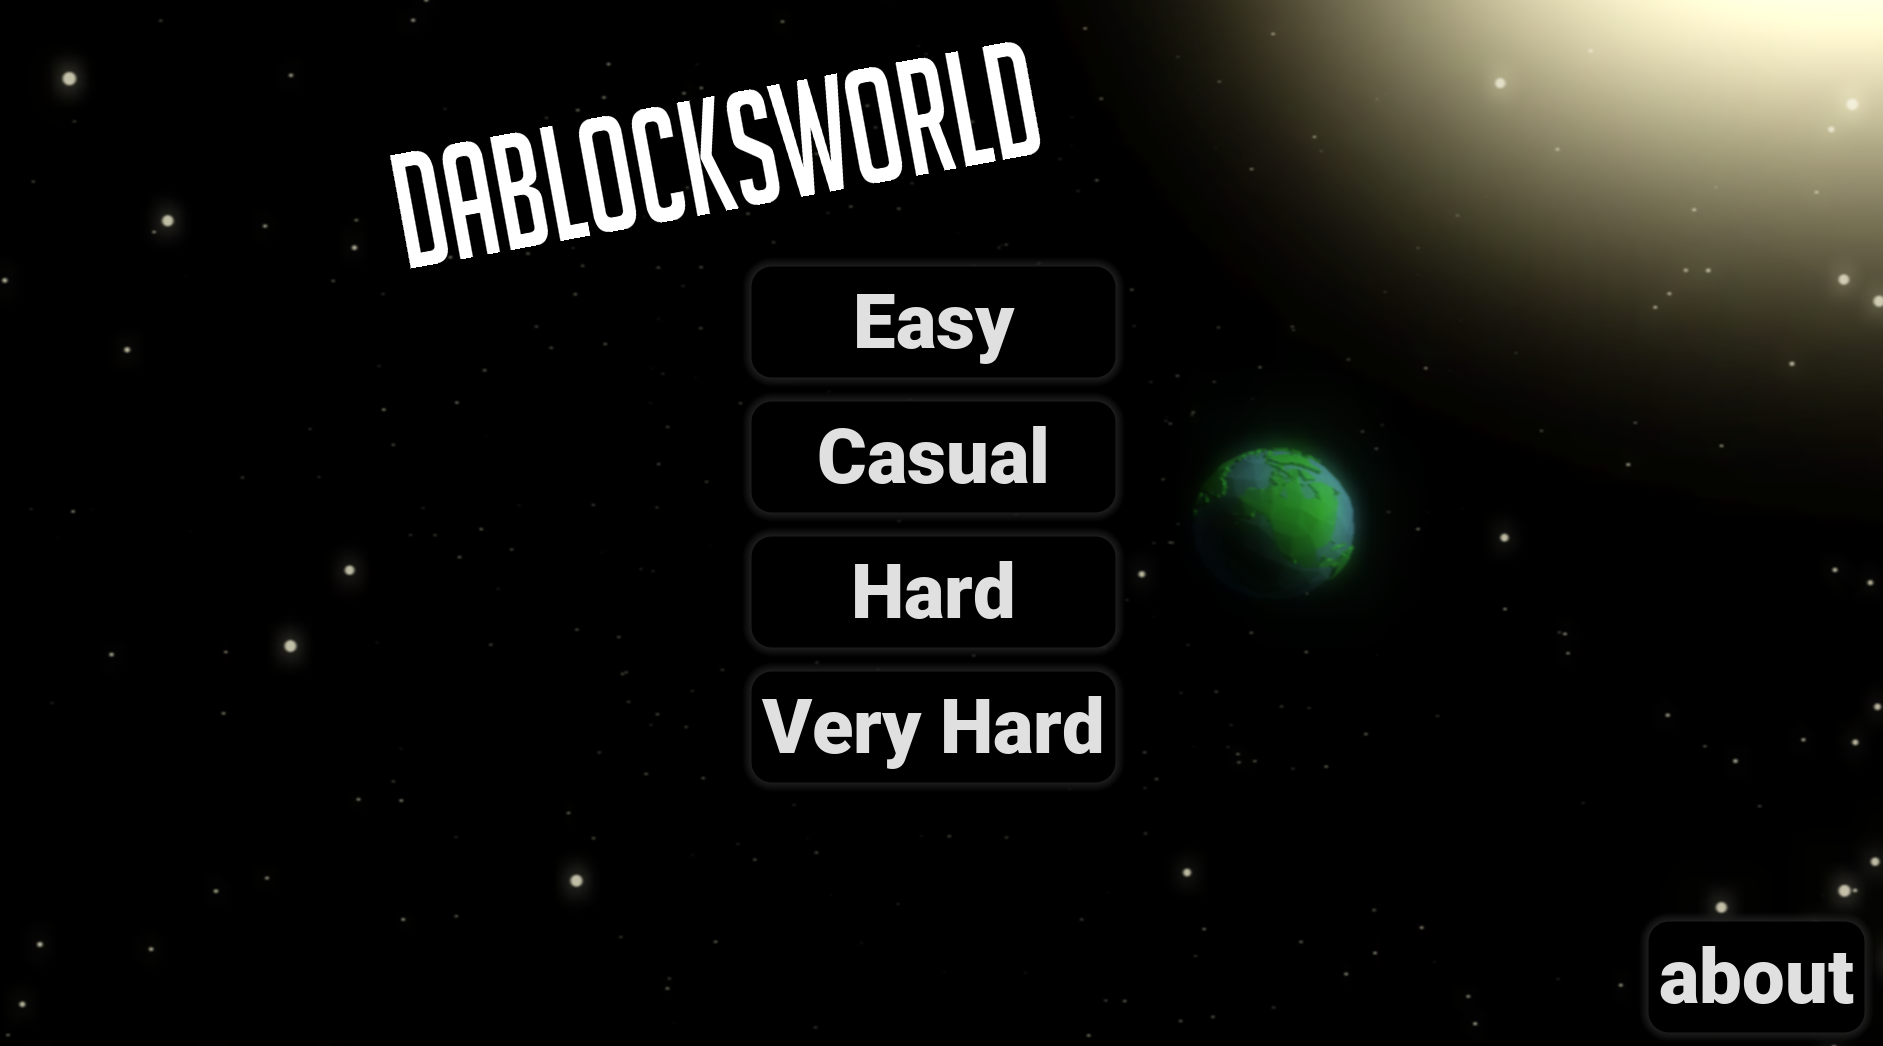
\includegraphics[width=\linewidth]{titleScreen.png}
                \label{titleScreen}
            \end{figure}
        \end{frame}

    \section{Solving BWPP}
        \begin{frame}[fragile]{Solving Configurations}
            \tiny
            \begin{lstlisting}
                #include <incmode>.
                #program base.
                % DOMAIN
                do(X,Z)   :- init(X,Y), not table(Y), table(Z).
                do(X,Y)   :- goal(X,Y), not table(Y).
                on(X,Y,0) :- init(X,Y).
                #program check(t).
                % TEST
                :- query(t), goal(X,Y),  not on(X,Y,t).
                #program step(t).
                % GENERATE
                1 {move(X,Y,t) : do(X,Y)} 1.
                % DEFINE
                move(X,t)   :- move(X,Y,t).
                on(X, Y, t) :- move(X,Y,t).
                on(X, Y, t) :- on(X,Y,t-1), not move(X,t).
                ...
            \end{lstlisting}
        \end{frame}
       
        \begin{frame}[fragile]
            \frametitle{Relevant moves}
            \begin{lstlisting}
                #program base.
                % DOMAIN
                do(X,Z)   :- init(X,Y), not table(Y), table(Z).
                do(X,Y)   :- goal(X,Y), not table(Y).
                on(X,Y,0) :- init(X,Y)
            \end{lstlisting}
        \end{frame} 

        \begin{frame}[fragile]
            \frametitle{Generating moves}
            \begin{lstlisting}
                #program step(t).
                % GENERATE
                1 {move(X,Y,t) : do(X,Y)} 1.
            \end{lstlisting}
        \end{frame}  

        \begin{frame}[fragile]{Needed height and width}
            \small
            \begin{lstlisting}
                blocksOnGround(A, t) :- #count{X :
                                               on(X, 0, t)} = A.
                height(B, 1, t) :- on(B, 0, t).
                height(B1, H+1, t) :- height(B2, H, t),
                                      on(B1, B2, t),
                                      amountOfBlocks(A), H < A.
            \end{lstlisting}
        \end{frame}
        
        \begin{frame}[fragile]
            \frametitle{The goal condition}
            \begin{lstlisting}
                #program check(t).
                % TEST
                :- query(t), goal(X,Y),  not on(X,Y,t).
            \end{lstlisting}
        \end{frame}

        \begin{frame}[fragile]
            \frametitle{Clingo's output}
            \begin{lstlisting}
                % DISPLAY
                #show move/3.
                #show blocksOnGround/2.
                #show height/3.
            \end{lstlisting}
        \end{frame}
    
    \section{Conclusion}
        \begin{frame}[fragile]
            \frametitle{Conclusion}
            \begin{itemize}
                \item ASP (AI) enables new game design aspects
                \item We could rate the performance of the player
                \item An algorithm without ASP would be larger
                      and most probably slower
            \end{itemize}
        \end{frame}

    %end
    \begin{frame}[fragile]{Questions}
        \begin{center}
            Questions?  
        \end{center}
    \end{frame}

    \begin{frame}[fragile]{Sources}
        \begin{itemize}
            \item \url{https://godotengine.org/}
            \item \url{https://potassco.org/clingo/}
            \item \url{https://github.com/CaptainDario/DaBlocksWorld}
            \item \url{https://aaai.org/ojs/index.php/aimagazine/article/view/2673}
            \item \url{https://pngio.com/images/png-a891433.html}
        \end{itemize}
    \end{frame}

    \begin{frame}[fragile]{Thank you}
        \begin{center}
            Thank you for your attention!
        \end{center}
    \end{frame}
\end{document}

